\chapter[Pravdepodobnosť a štatistika]{Pravdepodobnosť a štatistika}
\label{pravdepodobnost_a_statistika} % id kapitoly pre prikaz ref

(Predmety Pravdepodobnosť a štatistika, Integrácia dátových zdrojov, Metódy v bioinformatike)

\section{Definícia pravdepodobnostného modelu a základné vlastnosti pravdepodobnosti}

\subsection {sigma algebra}
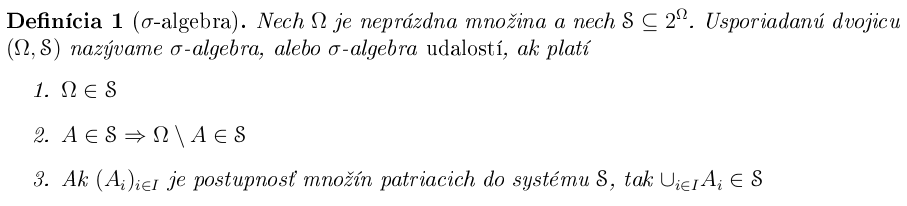
\includegraphics[width=1\textwidth]{images/pravdepodobnost/sigma_alg}\\
\subsection {pravdepodobnostná miera}
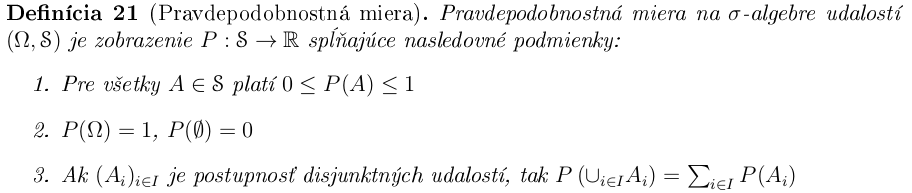
\includegraphics[width=1\textwidth]{images/pravdepodobnost/pravd_mier}\\
\subsection {princíp inklúzie-exklúzie}
pre udalosti A, B platí: $P (A \cup B) = P (A) + P (B) -- P (A \cap B)$\\
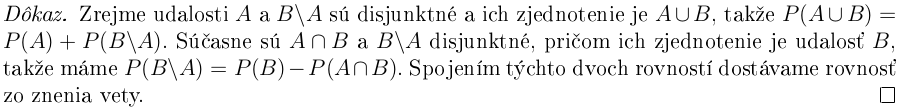
\includegraphics[width=1\textwidth]{images/pravdepodobnost/inklu_1}\\
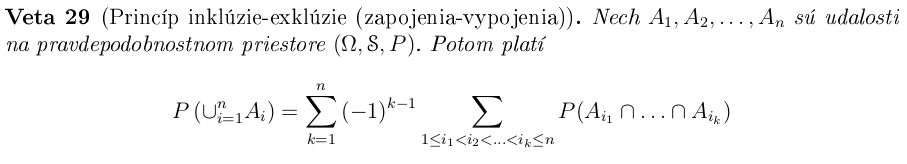
\includegraphics[width=1\textwidth]{images/pravdepodobnost/inkluzia_ex}\\

\section{Nezávislosť udalostí, podmienená pravdepodobnosť a Bayesove vety}

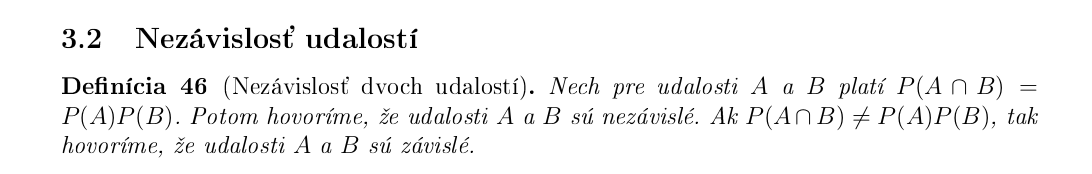
\includegraphics[width=1\textwidth]{images/pravdepodobnost/nezav_ud}\\
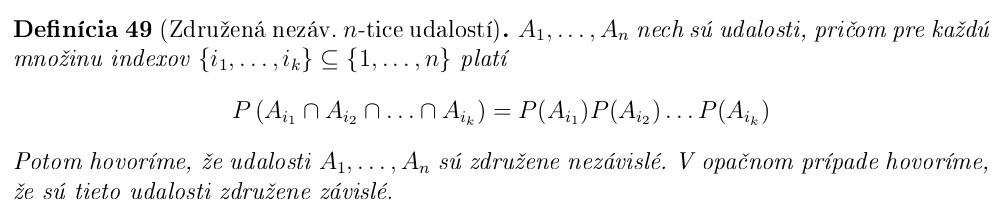
\includegraphics[width=1\textwidth]{images/pravdepodobnost/zdruz_nezav}\\
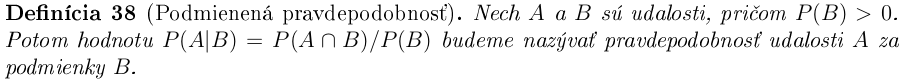
\includegraphics[width=1\textwidth]{images/pravdepodobnost/podmien_pravd}\\
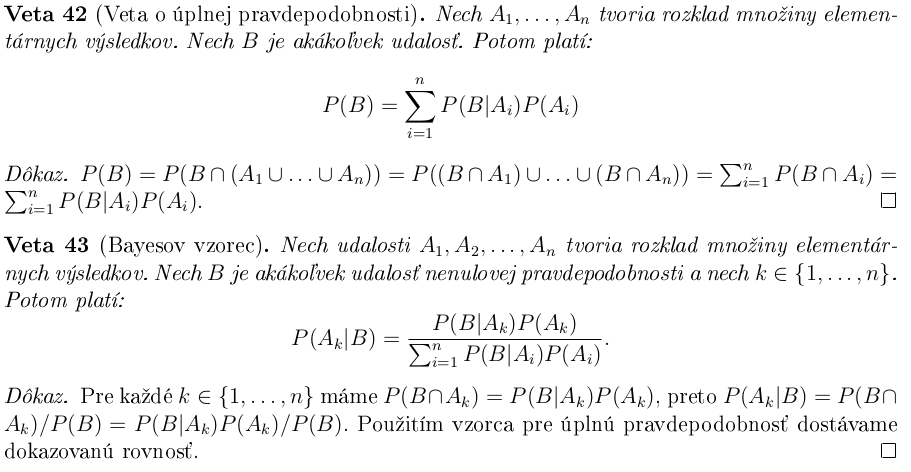
\includegraphics[width=1\textwidth]{images/pravdepodobnost/upln_pravd}\\

\section{Diskrétne náhodné premenné}

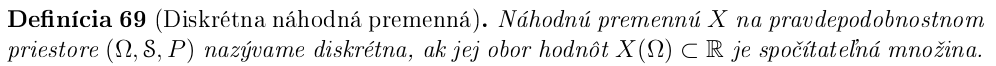
\includegraphics[width=1\textwidth]{images/pravdepodobnost/disk_nah_prem}\\
\subsection {distribučná funkcia}
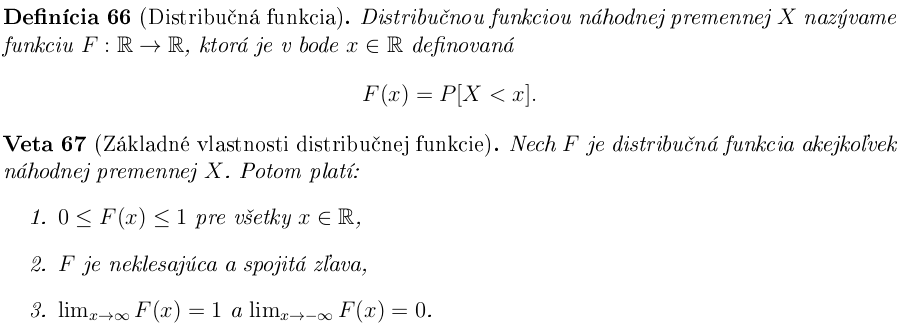
\includegraphics[width=1\textwidth]{images/pravdepodobnost/dist_funk}\\
\subsection {stredná hodnota}

\includegraphics[width=1\textwidth]{images/pravdepodobnost/stred_hod}\\
Linearita strednej hodnoty\\
\subsection {disperzia}
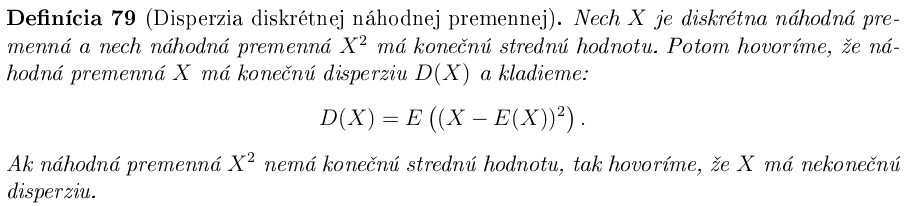
\includegraphics[width=1\textwidth]{images/pravdepodobnost/disp}\\
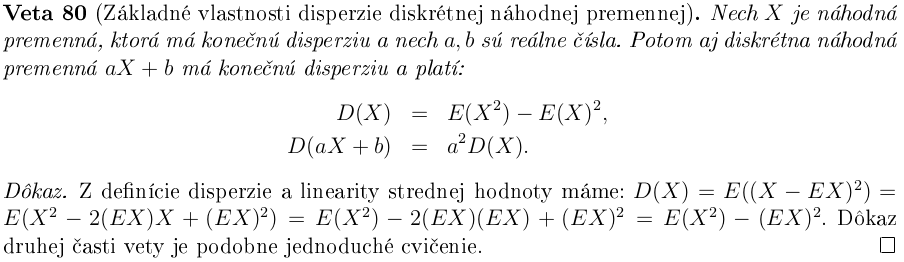
\includegraphics[width=1\textwidth]{images/pravdepodobnost/disp_II}\\
$D(X) = {x_1}^2.p_1 + {x_2}^2.p_2 + ... + {x_n}^2.p_n - (x_1.p_1 + x_2.p_2 + ... + x_n.p_n)^2$\\
\subsection {binomické, Poissonovo a geometrické rozdelenie}
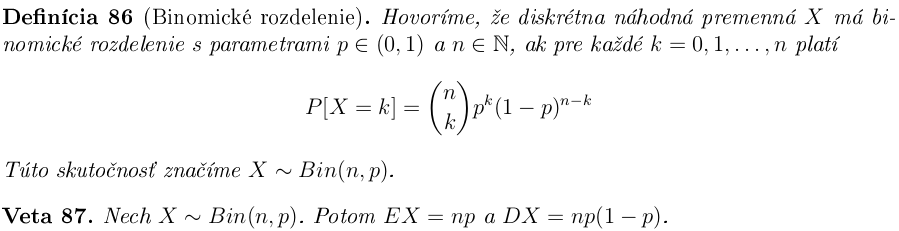
\includegraphics[width=1\textwidth]{images/pravdepodobnost/binom_rozd}\\
Opakovaný hod mincou (n-krát)\\
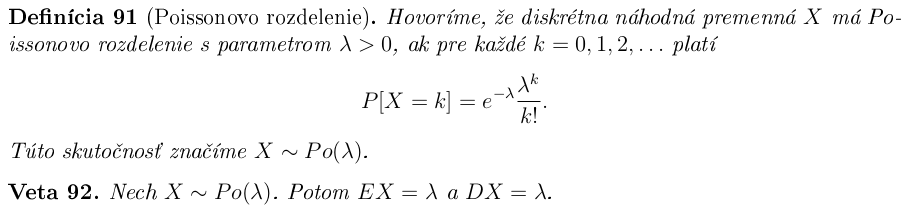
\includegraphics[width=1\textwidth]{images/pravdepodobnost/poiss_rozd}\\
aproximácia binomického rozdelenia\\
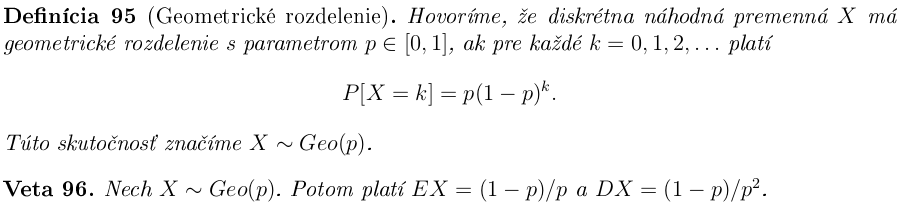
\includegraphics[width=1\textwidth]{images/pravdepodobnost/geom_rozd}\\
Počet hodov mincou (-1) kým nám nepadne hlava\\

\section{Spojité náhodné premenné}
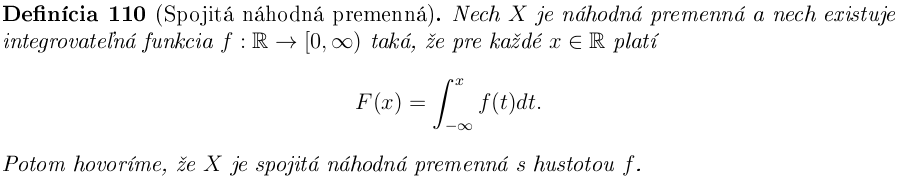
\includegraphics[width=1\textwidth]{images/pravdepodobnost/spoj_nah_prem}\\
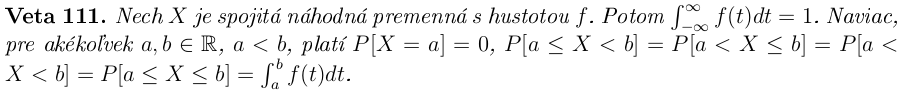
\includegraphics[width=1\textwidth]{images/pravdepodobnost/spoj_nah_prem_II}\\
\subsection {distribučná funkcia}
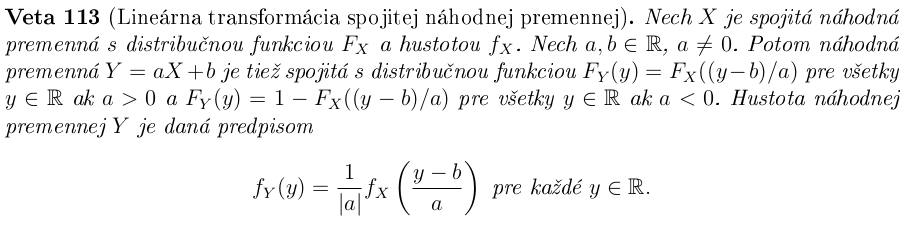
\includegraphics[width=1\textwidth]{images/pravdepodobnost/dist_funk_spoj}\\
\subsection {hustota}
To je tá funkcia z definície 110\\
\subsection {stredná hodnota}
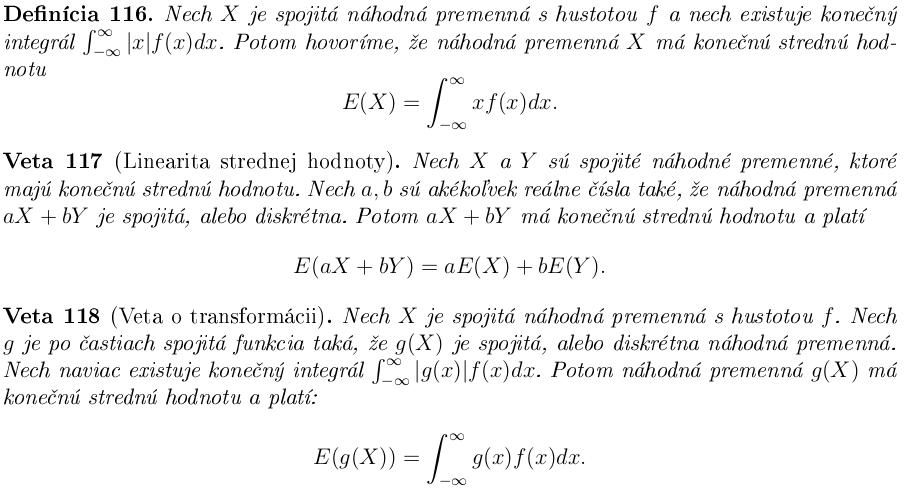
\includegraphics[width=1\textwidth]{images/pravdepodobnost/stred_hod_spoj}\\
\subsection {disperzia}
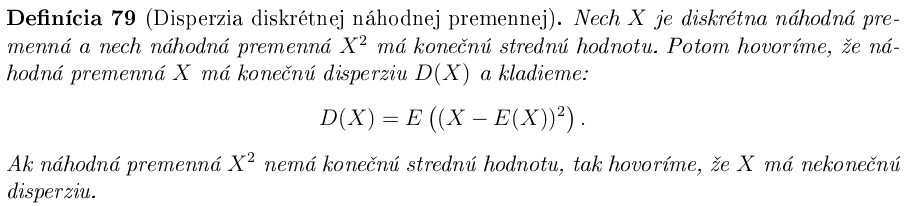
\includegraphics[width=1\textwidth]{images/pravdepodobnost/disp}\\
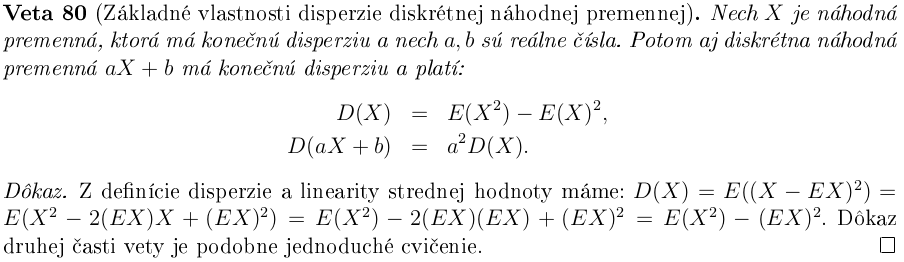
\includegraphics[width=1\textwidth]{images/pravdepodobnost/vlast_disp}\\
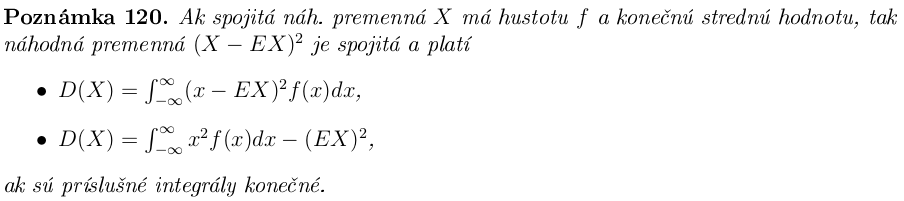
\includegraphics[width=1\textwidth]{images/pravdepodobnost/pozn_disp_spoj}\\
Integrovať od a po b namiesto -$\infty$ po $\infty$\\
\subsection {rovnomerné, exponenciálne a normálne rozdelenie}
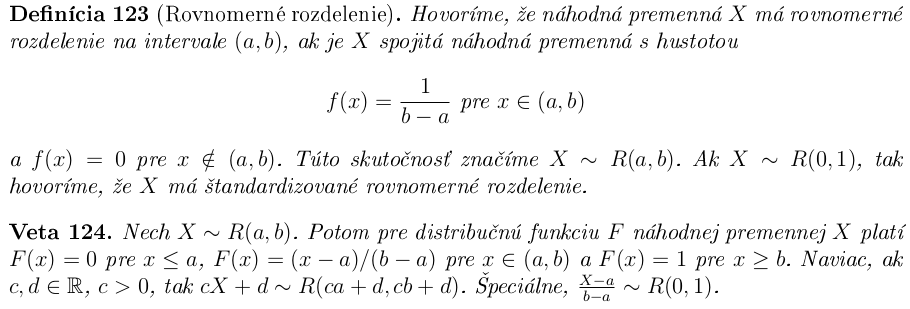
\includegraphics[width=1\textwidth]{images/pravdepodobnost/rovn_rozd}\\

\includegraphics[width=1\textwidth]{images/pravdepodobnost/rovn_rozd_II}

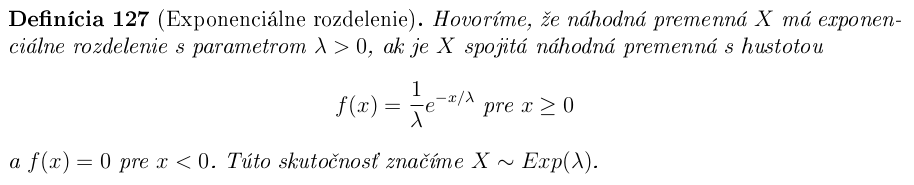
\includegraphics[width=1\textwidth]{images/pravdepodobnost/exp_rozd}\\

\includegraphics[width=1\textwidth]{images/pravdepodobnost/exp_rozd_II}

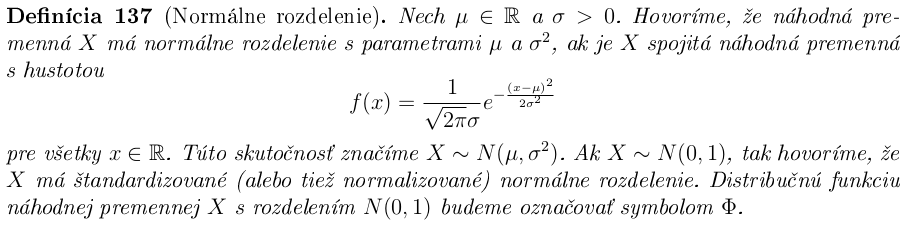
\includegraphics[width=1\textwidth]{images/pravdepodobnost/norm_rozd}\\

\includegraphics[width=1\textwidth]{images/pravdepodobnost/norm_rozd_II}\\

\section{Zákon veľkých čísel a limitné vety}

\subsection {Markovova a Čebyševova nerovnosť}
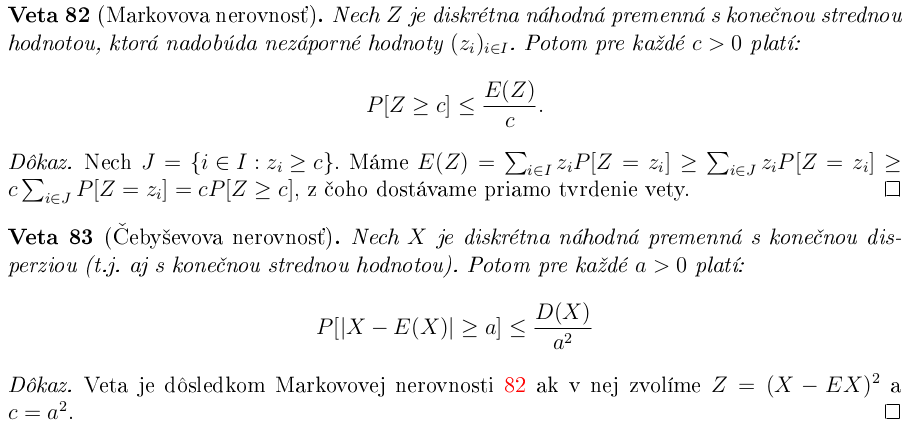
\includegraphics[width=1\textwidth]{images/pravdepodobnost/mark_cebys_ner}\\
\subsection {slabý zákon veľkých čísel}
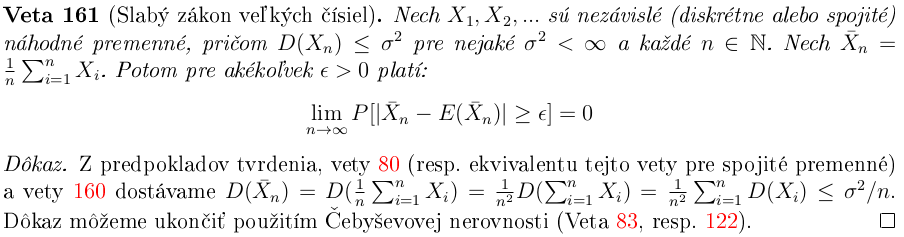
\includegraphics[width=1\textwidth]{images/pravdepodobnost/slaby_zak_velk_cis}\\
\subsection {centrálna limitná veta}
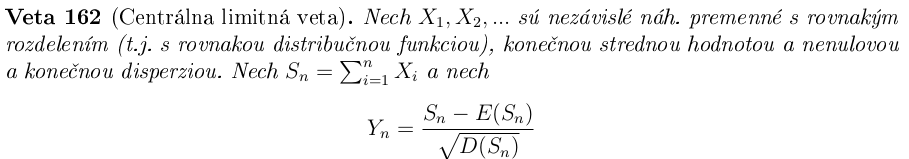
\includegraphics[width=1\textwidth]{images/pravdepodobnost/cent_lim_vet}\\

\section{Náhodné vektory}

\subsection {distribučná funkcia}
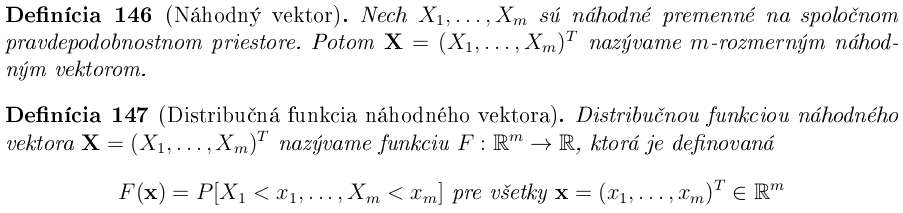
\includegraphics[width=1\textwidth]{images/pravdepodobnost/nah_vekt_dist_funk}\\
\subsection {nezávislosť náhodných premenných}
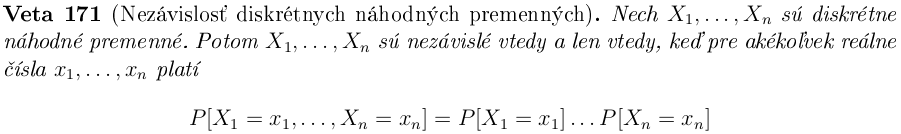
\includegraphics[width=1\textwidth]{images/pravdepodobnost/nezav_nah_prem}\\
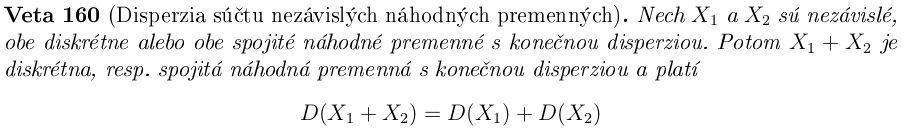
\includegraphics[width=1\textwidth]{images/pravdepodobnost/disp_nezav_nah_prem}\\
\subsection {kovariancia}
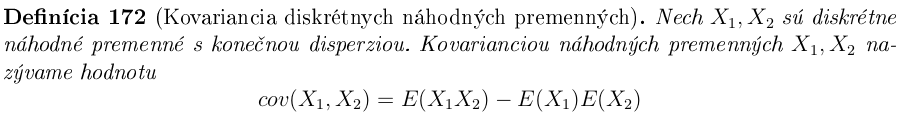
\includegraphics[width=1\textwidth]{images/pravdepodobnost/kovar}\\
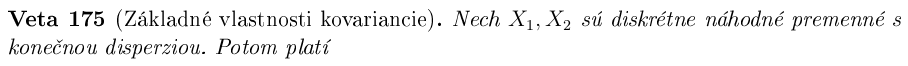
\includegraphics[width=1\textwidth]{images/pravdepodobnost/vlast_kovar}\\
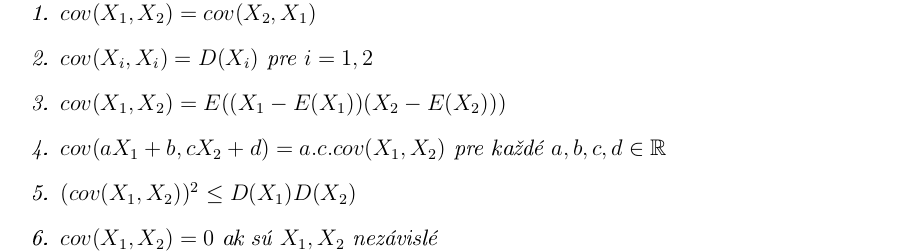
\includegraphics[width=1\textwidth]{images/pravdepodobnost/vlast_kovar_II}\\
\subsection {korelačný koeficient}
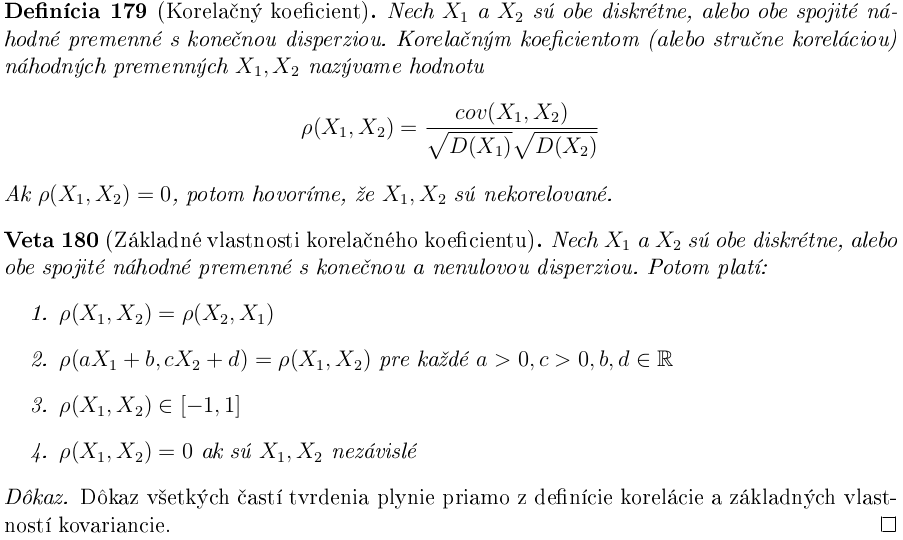
\includegraphics[width=1\textwidth]{images/pravdepodobnost/korel_koef}\\
\subsection {stredná hodnota}
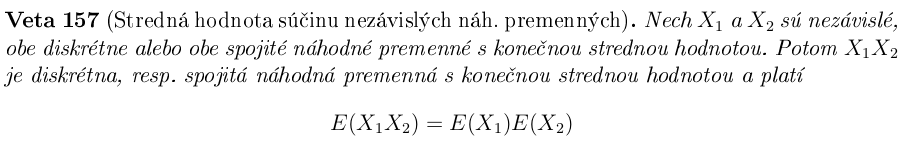
\includegraphics[width=1\textwidth]{images/pravdepodobnost/stred_hod_nah_prem}\\
\subsection {multinomické a viacrozmerné normálne rozdelenie}
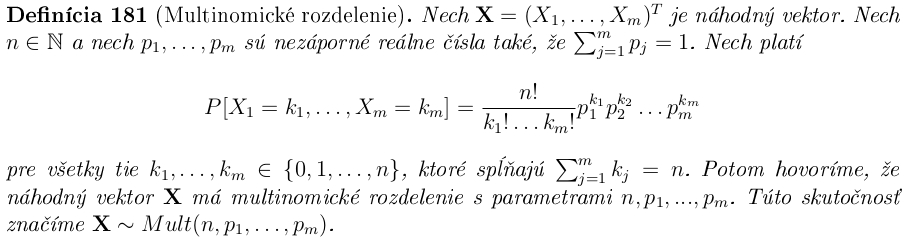
\includegraphics[width=1\textwidth]{images/pravdepodobnost/multinom_rozd}\\
Opakovaný hod kockou.\\
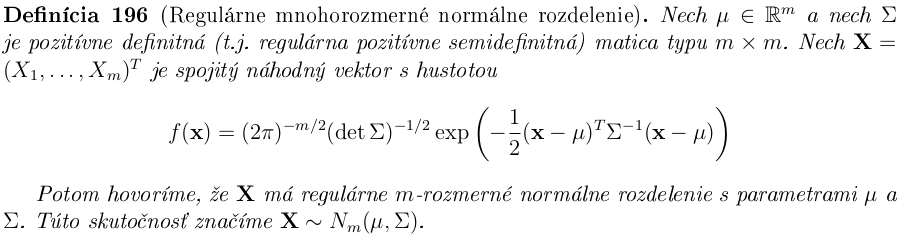
\includegraphics[width=1\textwidth]{images/pravdepodobnost/viacrozm_norm_rozd}\\

\section{Použitie štatistických testov}

\subsection {Fisherov exaktný test}
\subsection {chí-kvadrát test}
\subsection {Welchov t-test}
\subsection {Mann-Whitneyho U-test}
\subsection {Bonferroniho korekcia viacnásobného testovania}
